\documentclass{beamer}
\usetheme{HongKong}
\useinnertheme{rounded}
\usepackage{color, colortbl}
\usepackage{tcolorbox}
\usepackage{multirow}
\usepackage{textcomp}
\usepackage{siunitx}
\usepackage{tikz}
\usepackage[utf8]{inputenc}
\usepackage[safe]{tipa}

\tikzset{rndblock/.style={rounded corners,rectangle,draw,outer sep=0pt}}
\newcommand{\tframed}[2][]{\tikz[baseline=0.1pt]\vspace{0.1cm}\node[rndblock,minimum height=1.5em,#1] (m) {#2} ;}
\newcommand{\hilight}[1]{\textbf{\tframed[blue,fill=blue!10]{#1}}}
\newcommand{\whilight}[1]{\textbf{\tframed[purple,fill=purple!10]{#1}}}

\newcommand{\sP}{\hspace{1pt}}
\newcommand{\mP}{\hspace{3pt}}
\newcommand{\bP}{\hspace{6pt}}
\newcommand{\BP}{\hspace{12pt}}

%\newcommand{\hilight}[1]{\colorbox{white}{#1}}

%==============================================================================================================

\setbeamertemplate{navigation symbols}{}
\setbeamertemplate{items}[ball]
\setbeamertemplate{blocks}[rounded][shadow=true,width=.7\textwidth]

\setbeamercolor{myBlueBox} {bg=blendedblue, fg=white}
\setbeamercolor{myGrayBox} {bg=blendedgray, fg=black}

\definecolor{blendedblue}{rgb}{0.137,0.466,0.741}
\definecolor{blendedgray}{rgb}{0.838,0.833,0.833}
\definecolor{blendedpurple}{rgb}{0.147, 0.400, 0.700}
\definecolor{tgray}{rgb}{0.211, 0.211,0.244}
\definecolor{darkgray}{rgb}{0.450,0.450,0.450}
\definecolor{maroon}{rgb}{0.665, 0.142, 0.142}
\definecolor{ngreen}{rgb}{0.000,0.500,0.000}

\newcolumntype{g}{>{\columncolor{tgray}}S[tabformat=2.2]}

\newenvironment<>{varblock}[2][\textwidth]{%
\vspace*{-20pt}
	  \setlength{\textwidth}{#1}
	  \begin{actionenv}#3%
	    \def\insertblocktitle{#2}%
	    \par%
	    \usebeamertemplate{block begin}}
	  {\par%
	    \usebeamertemplate{block end}%
	  \end{actionenv}
\vspace*{-20pt}
}

%==============================================================================================================

\title{Comparison of approaches for an efficient phonetic decoding}

\author[Luiza Orosanu and Denis Jouvet]{Luiza Orosanu and Denis Jouvet \\
	\textcolor{polyured}{\tiny \textbf \{luiza.orosanu, denis.jouvet\}@loria.fr}}

\institute{Speech Group, LORIA\\Inria, Villers-les-Nancy, F-54600, France}
\date{August 27, 2013}

\AtBeginSection[]
{
  \begin{frame}
	\thispagestyle{empty}
   	\frametitle{Summary}
	\tableofcontents[currentsection,hideothersubsections,sectionstyle=show/shaded,subsectionstyle=hide] 	%currentsection,subsections, currentsubsection]
  \end{frame}
}

\newcommand{\firstslide}{%
	\begin{frame}
	\thispagestyle{empty}
	\titlepage
	\vspace{0.4cm}

	{\centering \linespread{0.4}\selectfont
	\tiny\color{darkgray}
	This study is part of the \textbf{\color{purple} RAPSODIE project} (http://erocca.com/rapsodie) and has received support from the "Conseil Régional de Lorraine" and from the "Région Lorraine" (FEDER)
	\par}
	\end{frame}
}

%==============================================================================================================
\begin{document}
\renewcommand{\inserttotalframenumber}{18}

%==============================================================================================================
\firstslide

%==============================================================================================================
%\begin{frame}
%	\frametitle{Summary}
%	\thispagestyle{empty}
%	\tableofcontents[currentsection,hideothersubsections,sectionstyle=show,subsectionstyle=hide] 		%currentsection,subsections, currentsubsection]
%\end{frame}

%==============================================================================================================
\section{Context and Considerations}
\begin{frame}{Context}
\setcounter{framenumber}{1}

\bigskip
\begin{center}
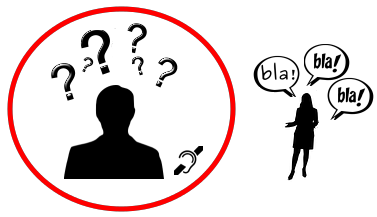
\includegraphics[scale=0.35]{Image/picture/deaf_support}
\end{center}

\begin{center}
\begin{itemize}
\item<1-> Deafness
	\begin{list}{$\ast$}{\leftmargin=4mm \itemindent=0em}
	\item {\scriptsize for \textbf{\color{purple} children}: can delay language development and cognitive skills}
	\item {\scriptsize for \textbf{\color{purple} adults}: difficulty to find an employment, exercise and keep it}
	\item {\scriptsize for \textbf{\color{purple} all}: social isolation}
	\end{list}
\end{itemize}
\bigskip

\begin{itemize}
\item<2> A speech recognition system adapted to deaf people's needs
	\begin{list}{$\ast$}{\leftmargin=4mm \itemindent=0em}
	\item {\scriptsize improve communication between deaf people and their entourage}
	\item {\scriptsize tool of socialization and/or integration in the workplace}
	\end{list}
\end{itemize}
\bigskip

\end{center}
\end{frame}


%==============================================================================================================
\begin{frame}{Considerations}

\begin{itemize}
\bigskip

\item<1-> Why consider a \textbf{\color{purple}portable solution} ?
	\begin{list}{$\ast$}{\leftmargin=4mm \itemindent=0em}
	\item[$\ast$] {\scriptsize could be used anywhere \& anytime}
	\item[$\ast$] {\scriptsize could give real-time information to its owner}
	\end{list}

\bigskip

\item<2> \textbf{\color{purple}Constraints} on considering an embedded device
	\begin{list}{$\ast$}{\leftmargin=4mm \itemindent=0em}
	\item[$\ast$] {\scriptsize limited memory size}
	\item[$\ast$] {\scriptsize limited computational power}
	\end{list}

\end{itemize}
\end{frame}

%==============================================================================================================
\section{Methodology}
\begin{frame}{Methodology}
\setcounter{framenumber}{3}
\bigskip

\begin{itemize}
\item<1-> \textbf{\color{purple} Objective}
{\footnotesize
$\ast \:\: \text{find the best compromise between} \;
\left\{
    \begin{array}{ll}
        \text{computational cost} \\
        \text{usability of results}
    \end{array}
\right.$
}

\vspace{0.8cm}

\item<2-> \textbf{\color{purple} Approaches}

\begin{list}{$\ast$}{\leftmargin=4mm \itemindent=0em}
{\footnotesize
\item always use the \textbf{\color{purple} same acoustic units}
\smallskip
\item evaluate \textbf{\color{purple} 3 different linguistic units} \\
	\hspace{1cm} $\Rightarrow$ different vocabularies \& different language models
}
\end{list}

\bigskip

\begin{table}[T]
\begin{tabular}{c|c}
\textbf{Acoustic unit}	& \textbf{Linguistic unit}	\\ \hline
			& phoneme			\\
phoneme			& syllable			\\
			& word				\\
\end{tabular}\hfill\
\end{table}


\end{itemize}
\end{frame}


%==============================================================================================================
\subsection{Comparison of Linguistic units}
\begin{frame}[t]{Comparison of linguistic units}

\vspace{0.1cm}
\begin{center}
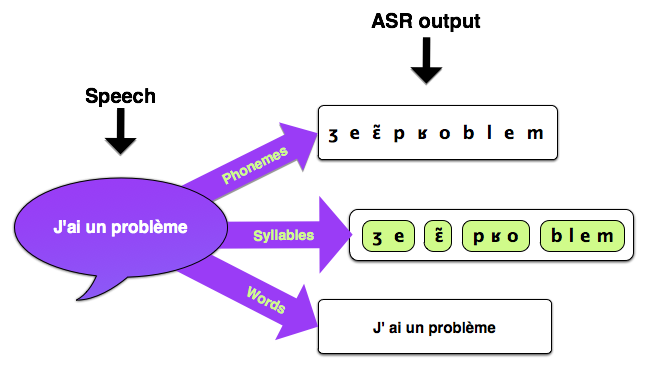
\includegraphics[scale=0.45]{Image/picture/lu}
\end{center}

\end{frame}


%==============================================================================================================
\begin{frame}[t]{Comparison of linguistic units}
\bigskip


\begin{list}{}{\leftmargin=4mm \itemindent=0em}
\item<1->
{
	\begin{columns}
	\begin{column}{.65\textwidth}
		\begin{itemize}
		\item phonemes
			\begin{list}{$\ast$}{\leftmargin=4mm \itemindent=0em}
				\item {\small vocabulary : $\textless$ 40 phonemes for French}
				\item {\small 3-gram language model : $\textless$ 1 MB}
			\end{list}
		\end{itemize}

	\end{column}
	\begin{column}{.35\textwidth}
		{\footnotesize \color{blendedblue}
		\begin{table}[t]
		\begin{tabular}{p{3.5cm}}
			\textbf{Lexicon entries}			\\ \hline
			au $\Rightarrow$ au				\\
			b  $\Rightarrow$ b				\\
			ge $\Rightarrow$ ge				\\
		\end{tabular}
		\end{table}
		}
	\end{column}
	\end{columns}
	\vfill
}

\item<3->
{
	\begin{columns}
	\begin{column}{.65\textwidth}
		\begin{itemize}
		\item \textbf{\color{purple}syllables}
			\begin{list}{$\ast$}{\leftmargin=4mm \itemindent=0em}
				\item {\small vocabulary : $\sim$ 16,000 syllables}
				\item {\small 3-gram language model : $\textless$ 10 MB}
			\end{list}
		\end{itemize}
	\end{column}
	\begin{column}{.35\textwidth}
		{\footnotesize \color{blendedblue}
		\begin{table}[t]
		\begin{tabular}{p{3.5cm}}
			\hline
			au\_s    $\Rightarrow$ au s				\\
			b\_l\_au $\Rightarrow$ b l au 				\\
			o\_r     $\Rightarrow$ o r 				\\
		\end{tabular}
		\end{table}
		}
	\end{column}
	\end{columns}
}



\item<2->
{
	\begin{columns}
	\begin{column}{.65\textwidth}
		\begin{itemize}
		\item words
			\begin{list}{$\ast$}{\leftmargin=4mm \itemindent=0em}
				\item {\small vocabulary : $\sim$ 97,000 words}
				\item {\small 3-gram language model: $\textgreater$ 1 GB}
			\end{list}
		\end{itemize}
	\end{column}
	\begin{column}{.35\textwidth}
		{\footnotesize \color{blendedblue}
		\begin{table}[t]
		\begin{tabular}{p{3.5cm}}
			\hline
			absent   $\Rightarrow$ 	a b s an		\\
			combiner $\Rightarrow$  k on b i n e		\\
			libre    $\Rightarrow$ 	l i b r			\\
		\end{tabular}
		\end{table}
		}
	\end{column}
	\end{columns}
}
\end{list}
\vspace{1cm}
\end{frame}

%==============================================================================================================
\subsection{The syllables}
\begin{frame}[t]{Syllables}
\bigskip

\begin{itemize}
\item<1-> Setup for \textbf{\color{purple}defining the syllables}
	\begin{list}{$\ast$}{\leftmargin=12mm \itemindent=0em}
	\item {\scriptsize the training corpora is entirely \textbf{\color{purple}phonetized} (by forced alignment)}
	\item {\scriptsize the sequence of phonemes is processed by the \textbf{\color{purple}syllabification tool} }
	\end{list}

\smallskip

\item<2-> Rules of syllabification {\color{blendedblue}\scriptsize[Bigi et al,2010]}
	\begin{list}{$\ast$}{\leftmargin=12mm \itemindent=0em}
	\item {\scriptsize a syllable contains a single vowel {\color{gray}(V)}}
	\item {\scriptsize a pause designates a syllable's boundary}
	\end{list}

\bigskip

\only<3>
{
\footnotesize
\begin{table}[T]
\begin{tabular}{r|c|l}
\textbf{Sequence of phonemes} & \textbf{Split position} & \textbf{Resulting syllables} 		\\ \hline
VV 		& 0 & \ \ \ \ V \ \ \ V	 	\\
VxV 		& 0 & \ \ \ \ V \ \- xV		\\
VxxV 		& 1 & \ \- \- Vx \ \- xV			\\
VxxxV 		& 2 & \- \- Vxx  \ \- xV	 		\\
\end{tabular}
\end{table}
\vspace{-2.05cm}
}


\vspace{2.4cm}

\only<2->
{
\color{blendedblue}
\rule{40mm}{0.5pt}\\
\linespread{0.4}\selectfont
\tiny [Bigi et al.,2010] Bigi, B., Meunier, C., Bertrand, R. and Nesterenko, I., "Annotation automatique en syllabes d'un dialogue oral spontané", Journées d'Étude de la Parole, 2010
\par
}


\end{itemize}
\end{frame}

%==============================================================================================================
\begin{frame}[t]{Syllables}
\bigskip
\smallskip

%\only<1->
%{
%\begin{beamerboxesrounded}{Example 1}
%\textbf{\footnotesize les \BP\BP derniers \mP\bP\BP\BP sondages}

%\textbf{\footnotesize \textipa{l} \sP \textipa{e} \sP\BP \textipa{d} \mP \textepsilon \bP \textinvscr \bP \textipa{n} \mP \textipa{j} \mP e \sP\sP\BP s \mP \~\textopeno \bP d \mP a \mP \textyogh} 		  \hspace{1.6cm} \textbf{\footnotesize\color{blendedblue} $\leftarrow$ forced alignment}

%\vspace{0.1cm}
%\hilight{l\_\textipa{e}} \bP \hilight{d\_\textepsilon\_\textinvscr} \sP \hilight{n\_j\_e} \BP \hilight{s\_\~\textopeno} \sP \hilight{d\_a\_\textyogh}	  \hspace{1.55cm} \textbf{\footnotesize\color{blendedblue} $\leftarrow$ syllables}
%\end{beamerboxesrounded}
%}

\bigskip
\only<1->
{
\begin{beamerboxesrounded}[width=.9\textwidth,shadow=true]{Example}
\textbf{ {\color{maroon} ce \sP qui} \bP s' est \sP  passé \bP {\color{maroon} c' est \sP que} \bP {\color{gray} (...)}}

\textbf{
\textipa
{
{\color{maroon} s \sP k \sP i}
\bP s \mP e \mP p \mP a \mP s \mP e \bP
{\color{maroon} \mP s \sP e \sP k}
\hspace{1.1cm} {\color{blendedblue} $\leftarrow$ forced alignment}
}
}

\vspace{0.1cm}
\textipa{
\whilight{s\_k\_i} \sP \hilight{s\_e} \hilight{p\_a} \hilight{s\_e} \mP \whilight{s\_e\_k}
\hspace{0.6cm} \textbf{\normalsize \color{blendedblue} $\leftarrow$ syllables}}
\end{beamerboxesrounded}
}

\bigskip

\only<2>
{
\bigskip
\small
\begin{list}{$\Rightarrow$}{\leftmargin=4mm \itemindent=0em}
 	\item The syllabification tool creates \textbf{\color{blue}syllables} and \textbf{\color{maroon}pseudo-syllables}, which
	\begin{list}{$\ast$}{\leftmargin=12mm \itemindent=0em}
		\item take into account the \textbf{\color{blendedblue}liaison \& reduction} events
		\vspace{0.1cm}
		\item are consistant throughout the entire training data
	\end{list}
\end{list}
}

\end{frame}

%==============================================================================================================
\begin{frame}[t]{Syllables}

\begin{center}
	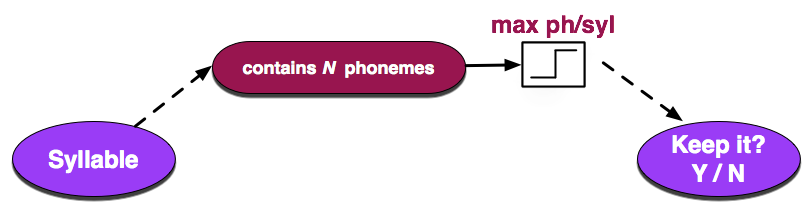
\includegraphics[scale=0.35]{Image/picture/filters_1}
\end{center}

\vspace{1.32cm}

\begin{itemize}
\item \small{Reduce the number of (pseudo-)syllables by applying \textbf{two filters}}
	\begin{list}{$\ast$}{\leftmargin=12mm \itemindent=0em}
	\item \small{a \textbf{\color{maroon} maximum number of phonemes} per syllable}
	\end{list}

\end{itemize}
\end{frame}

%==============================================================================================================
\begin{frame}[t]{Syllables}
\setcounter{framenumber}{8}

\vspace{1.35cm}

\begin{center}
	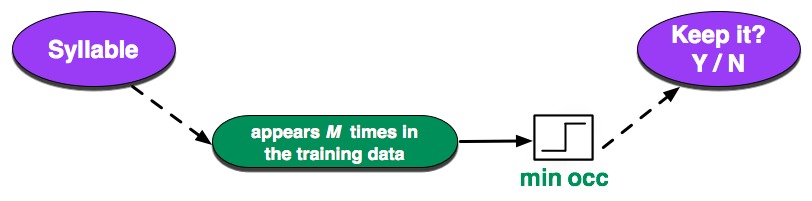
\includegraphics[scale=0.35]{Image/picture/filters_2}
\end{center}

\vspace{0.01cm}
\smallskip

\begin{itemize}
\item \small{Reduce the number of (pseudo-)syllables by applying \textbf{two filters}}
	\begin{list}{$\ast$}{\leftmargin=12mm \itemindent=0em}
	\vspace{0.43cm}
	\item \small{a \textbf{\color{ngreen} minimum number of occurrences} in the training data}
	\end{list}

\end{itemize}
\end{frame}

%==============================================================================================================
\begin{frame}[t]{Syllables}
\setcounter{framenumber}{8}

\begin{center}
	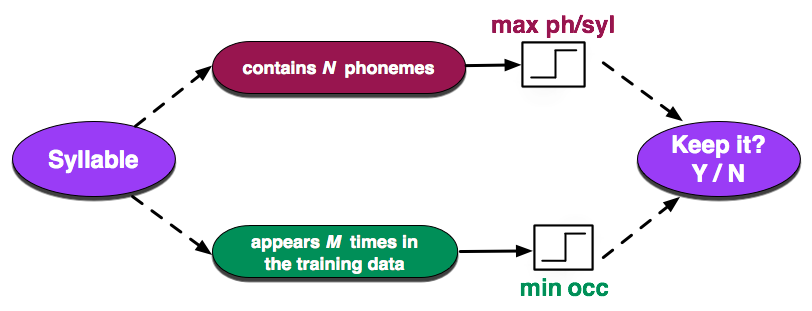
\includegraphics[scale=0.35]{Image/picture/filters}
\end{center}

\smallskip

\begin{itemize}
\item \small{Reduce the number of (pseudo-)syllables by applying \textbf{two filters}}
	\begin{list}{$\ast$}{\leftmargin=12mm \itemindent=0em}
	\item \small{a \textbf{\color{maroon} maximum number of phonemes} per syllable}
	\item \small{a \textbf{\color{ngreen} minimum number of occurrences} in the training data}
	\end{list}

\bigskip
$\Rightarrow$ create several different \textbf{lists of syllables}, by applying different thresholds for \textbf{each filter}

\end{itemize}
\end{frame}


%==============================================================================================================
%\begin{frame}{Comparison of Language Models}

%\bigskip
%\begin{table}[T]
%\begin{tabular}{|lc||S[tabformat=2.1]|S[tabformat=2.2]|S[tabformat=2.2]|S[tabformat=4.2]|}
%\hline
%\multirow{2}{*}{\textbf{LM}} & \multirow{2}{*}{} & \multicolumn{3}{c|}{\textbf{\# of n-grams}} & \multicolumn{1}{c|}{\textbf{Size}} 	 	\\ \cline{3-5}
%		& & \multicolumn{1}{c|}{\textbf{n=1}} & \multicolumn{1}{c|}{\textbf{n=2}} & \multicolumn{1}{c|}{\textbf{n=3}}	& \multicolumn{1}{c|}{\textbf{[MB]}}	\\ \hline \hline
%\multicolumn{2}{|c||}{\textbf{phonemes}}     & \multicolumn{1}{c|}{40}  & \multicolumn{1}{c|}{1347}	& \multicolumn{1}{c|}{30898} 	& 0.21	\\ \hline \hline
%\multirow{2}{*}{\textbf{syllables}} & \multicolumn{1}{|c||}{min4occ} 	& 7.2 K		& 0.37 M	& 1.73 M	& 9.90			\\
% & \multicolumn{1}{|c||}{max4ph}					& 13.4 K	& 0.38 M	& 1.73 M	& 10.14			\\ \hline \hline
%\multicolumn{2}{|c||}{\textbf{words}} 					& 97.3 K	& 43.35 M	& 79.30 M	& 1269.81		\\ \hline
%\end{tabular}
%\end{table}

%\end{frame}



%==============================================================================================================
\section{Experiments and results}
\begin{frame}[b]{Experiments}
\setcounter{framenumber}{9}
\begin{minipage}[.6\textheight]{\textwidth}
\begin{itemize}
\item use a single type of \textbf{\color{purple}acoustic unit}
	\begin{list}{$\ast$}{\leftmargin=12mm \itemindent=0em}
		\item {\color{blendedblue} the phoneme}
	\end{list}
\vspace{0.1cm}
\item use three different \textbf{\color{purple}linguistic units} ({\footnotesize $\Rightarrow$ diffent vocabularies \& LMs})
	\begin{list}{$\ast$}{\leftmargin=12mm \itemindent=0em}
		\item {\color{blendedblue}the phoneme}
		\item {\color{blendedblue}the syllable}
		\item {\color{blendedblue}the word}
	\end{list}
\vspace{0.1cm}
\item test them on two French speech corpora
\vspace{0.1cm}
\item study their phonetic decoding performance (PER)
\end{itemize}
\end{minipage}

\vfill
{\color{darkgray}\rule{40mm}{0.5pt}\\
\scriptsize{LM \ = Language model} \\
\scriptsize{PER = Phonemes Error Rate}}
\vspace{0.5cm}

\end{frame}

%==============================================================================================================
\begin{frame}[t]{Data for Acoustic training}
\vspace{0.8cm}

\begin{itemize}
\item \textbf{\color{purple}Train phonetic acoustic models}:
\begin{columns}
\begin{column}{.55\textwidth}
   	\begin{list}{$\ast$}{\leftmargin=17mm \itemindent=0em}
 	\item \footnotesize{ESTER2 train set}
 	\item \footnotesize{ETAPE train set}
 	\item \footnotesize{EPAC train set}
 	\end{list}
\end{column}
{\vrule height 0.5cm width 0.4pt}
\begin{column}{.45\textwidth}
 	\begin{itemize}
 	\item[$\Rightarrow$]  300h
 	\end{itemize}
\end{column}
\end{columns}
\end{itemize}

\vspace{1cm}
\only<2->
{
\scriptsize
\begin{columns}
\begin{column}{.30\textwidth}
\flushright \textbf{\color{blendedblue} ESTER2 \& EPAC}
\end{column}
{\vrule height 0.3cm width 0.4pt}
\begin{column}{.70\textwidth}
   	\begin{list}{$\ast$}{\leftmargin=3mm \itemindent=0em}
		\item French broadcast news, collected from radio channels
		\item prepared speech, plus interviews
	\end{list}
\end{column}
\end{columns}

\bigskip

\begin{columns}
\begin{column}{.30\textwidth}
\flushright \textbf{\color{blendedblue} ETAPE}
\end{column}
{\vrule height 0.3cm width 0.4pt}
\begin{column}{.70\textwidth}
   	\begin{list}{$\ast$}{\leftmargin=3mm \itemindent=0em}
		\item debates collected from various radio and TV channels
		\item spontaneous speech
	\end{list}
\end{column}
\end{columns}
}

\end{frame}


%==============================================================================================================
\subsection{Data}
\begin{frame}[t]{Data for LM training}

\smallskip
\begin{itemize}
\item \textbf{\color{purple} phoneme-based and syllable-based LM} \\
		\hspace{1cm}{\footnotesize\color{blendedblue} $\rightarrow$ training from phonetic transcription}
\begin{columns}
\begin{column}{.55\textwidth}
   	\begin{list}{$\ast$}{\leftmargin=20mm \itemindent=0em}
 	\item \footnotesize{ESTER2 train set}
 	\item \footnotesize{ETAPE train set}
 	\item \footnotesize{EPAC train set}
 	\end{list}
\end{column}
{\vrule height 0.5cm width 0.4pt}
\begin{column}{.45\textwidth}
 	\begin{itemize}
 	\item[$\Rightarrow$] 12 million phonemes
 	\item[$\Rightarrow$] 6 million syllables
 	\end{itemize}
\end{column}
\end{columns}

\only<2>
{
\bigskip
\begin{center}
\rule{100mm}{1.2pt}
\end{center}
\smallskip

\item \textbf{\color{purple} word-based LM} \\
	\hspace{1cm} {\footnotesize\color{blendedblue}$\rightarrow$ training from textual data}
\begin{columns}
\begin{column}{.55\textwidth}
   	\begin{list}{$\ast$}{\leftmargin=20mm \itemindent=0em}
	\item \footnotesize{newspaper data}
	\item \footnotesize{radio broadcast shows}
	\item \footnotesize{French Gigaword corpus}
	\item \footnotesize{web sources}
	\end{list}
\end{column}
{\vrule height 0.7cm width 0.4pt}
\begin{column}{.45\textwidth}
	\begin{itemize}
	\item[$\Rightarrow$] more than 1.5 billion words
	\end{itemize}
\end{column}
\end{columns}

}

\end{itemize}
\end{frame}




%#########################################################################
\begin{frame}[t]{Data for Evaluation}

\vspace{1.5cm}

\begin{itemize}
\item \textbf{\color{purple} Test} on:

\only<1->
{
\begin{columns}
\begin{column}{.55\textwidth}
   	\begin{list}{$\ast$}{\leftmargin=17mm \itemindent=0em}
 	\item ESTER2 development set \\
		\hspace{0.8cm}{\scriptsize\color{blendedblue}(prepared speech)}
 	\end{list}
\end{column}
{\vrule height 0.3cm width 0.4pt}
\begin{column}{.45\textwidth}
 	\begin{itemize}
	\item[$\Rightarrow$]  142,000 phonemes
 	\end{itemize}
\end{column}
\end{columns}
}

\smallskip

\only<2->
{
\begin{columns}
\begin{column}{.55\textwidth}
   	\begin{list}{$\ast$}{\leftmargin=17mm \itemindent=0em}
 	\item ETAPE development set \\
		\hspace{0.5cm}{\scriptsize\color{blendedblue}(spontaneous speech)}
 	\end{list}
\end{column}
{\vrule height 0.3cm width 0.4pt}
\begin{column}{.45\textwidth}
 	\begin{itemize}
	\item[$\Rightarrow$]  263,000 phonemes
 	\end{itemize}
\end{column}
\end{columns}
}

\end{itemize}
\end{frame}


%==============================================================================================================
\subsection{Configuration}
\begin{frame}[t]{Configuration}

\bigskip

\begin{itemize}
	\item<1-> SRILM tools \\
		\hspace{1cm} $\ast$ build statistical Language Models
	\bigskip

	\item<2-> MFCC acoustic analysis \\\
		\hspace{1cm} $\ast$ compute 13 MFCC parameters per frame
	\bigskip

	\item<3-> Sphinx3 tools \\
		\hspace{1cm} $\ast$ train phonetic acoustic models \\
			\hspace{2cm} {\scriptsize $\Rightarrow$ Context dependent HMM acoustic models}\\
				\hspace{3.5cm} $\left\{
                                     \begin{array}{ll}
                			\text{\scriptsize 64 Gaussian mixtures}    	\\
        		        	\text{\scriptsize 7500 senones}			\\
					\text{\scriptsize adapted Male/Female}
                                	\end{array}
                                \right.$ \\
		\smallskip
		\hspace{1cm} $\ast$ decode audio signals
\end{itemize}
\end{frame}

%==============================================================================================================
\subsection{Results}


%==============================================================================================================
\begin{frame}[b]{\textbf{\normalsize Results on the syllable-based LMs:} {\scriptsize\color{white} filter by a maximum number of ph/syl}}

\begin{center}
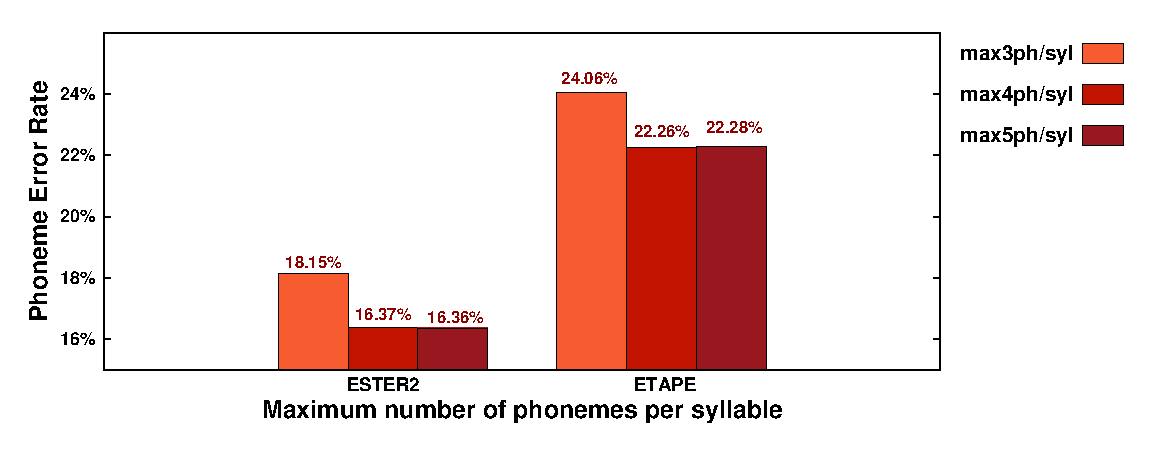
\includegraphics[scale=0.58]{Image/results/results_maxph}\\
\bigskip
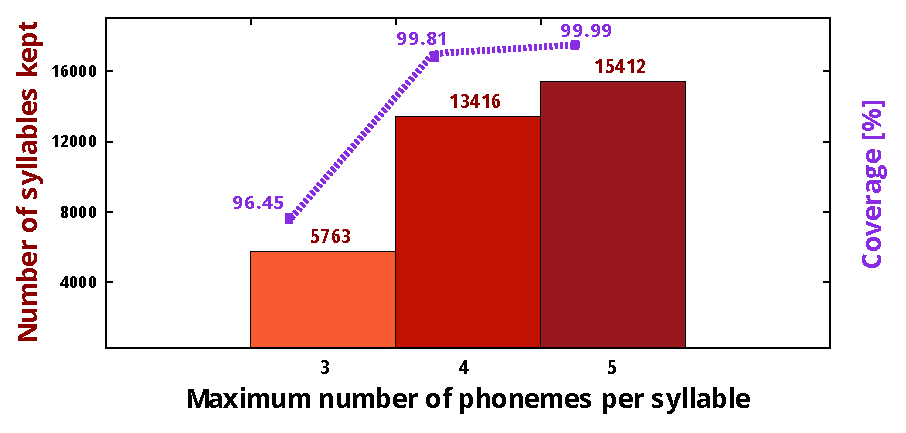
\includegraphics[scale=0.47]{Image/results/couverture_maxph_2in1}
\end{center}


\end{frame}


%==============================================================================================================
\begin{frame}[b]{\textbf{\normalsize Results on the syllable-based LMs:} {\scriptsize\color{white} filter by a minimum number of occurrences}}

\only<1>
{
	\begin{center}
	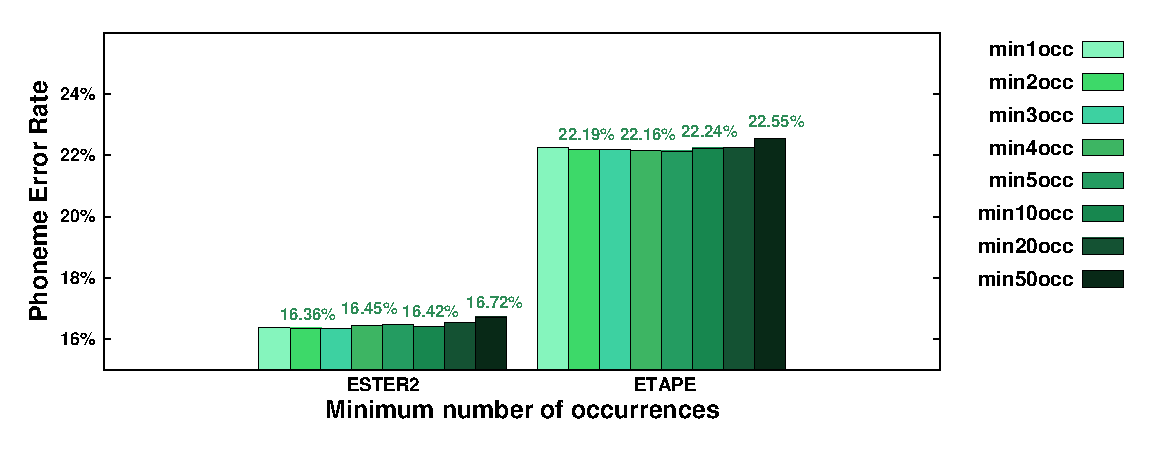
\includegraphics[scale=0.58]{Image/results/results_minocc}\\
	\bigskip
	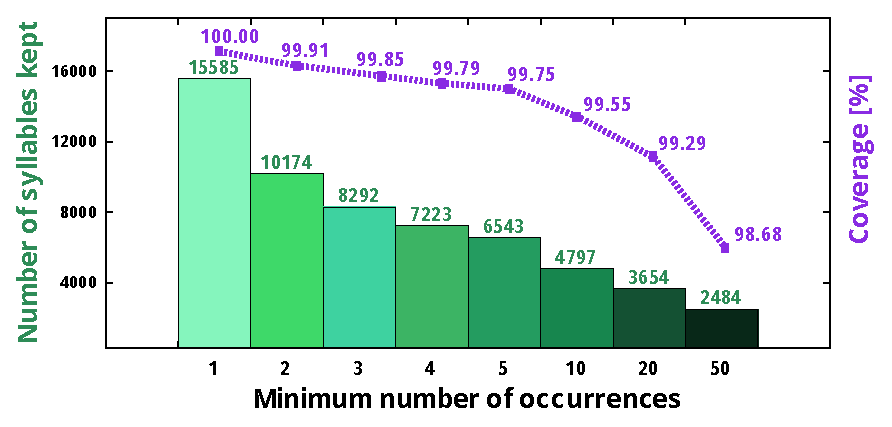
\includegraphics[scale=0.47]{Image/results/couverture_minocc_2in1}
	\end{center}
%	\vspace{1.01cm}
}

\only<2->
{
	\begin{center}
	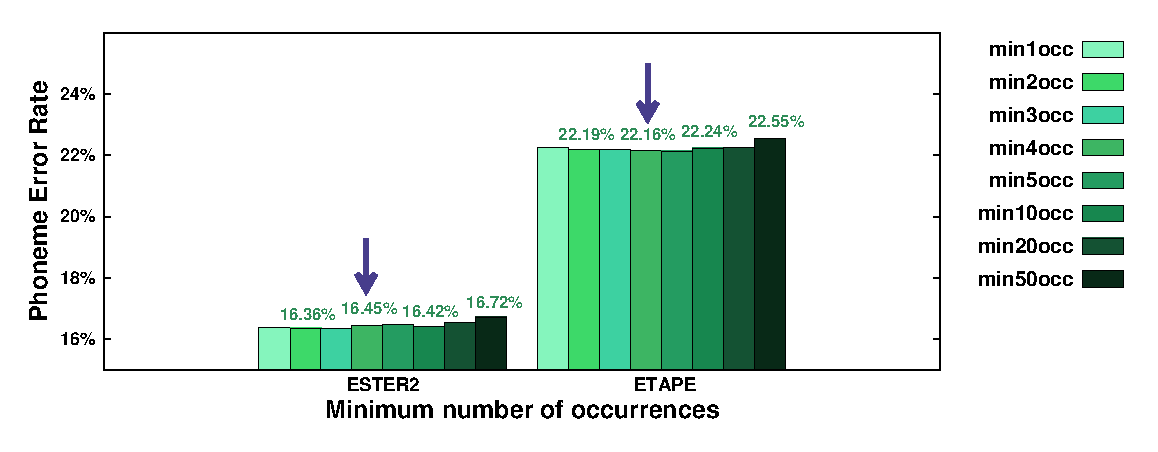
\includegraphics[scale=0.58]{Image/results/results_minocc_witharrow}\\
	\bigskip
	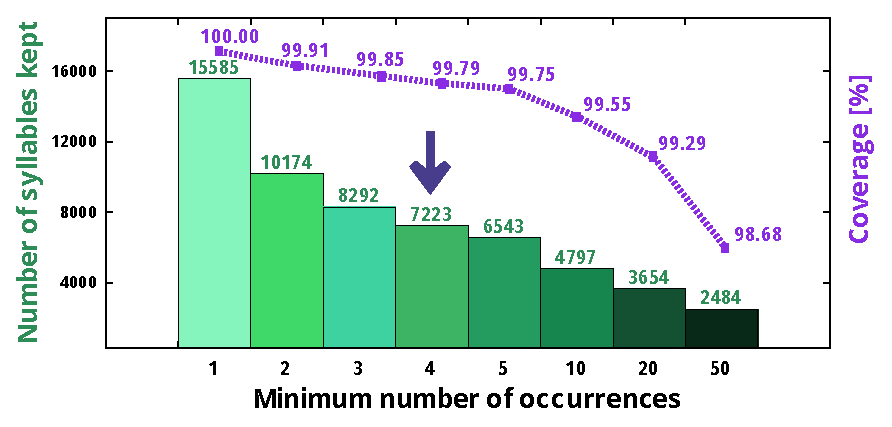
\includegraphics[scale=0.47]{Image/results/couverture_minocc_2in1_witharrow}
	\end{center}

%	\vfill
%	{\hspace{-0.5cm} \color{blendedblue}\rule{40mm}{0.5pt}\\
%	\hspace{-0.5cm} \textbf{\scriptsize A good compromise is the LM based on syllables seen at least 4 times during training}}
}

\end{frame}



%==============================================================================================================
\begin{frame}{Overall results}
\smallskip

\begin{center}
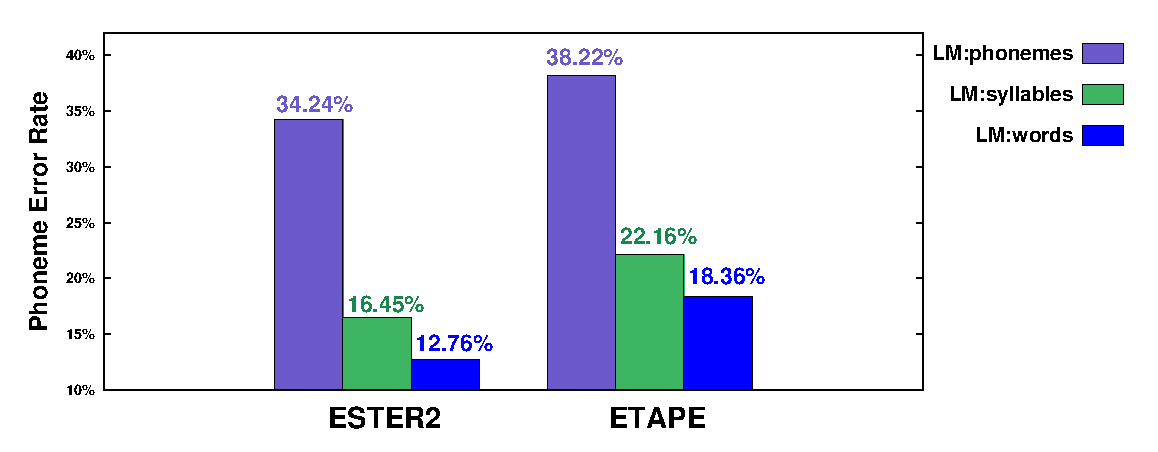
\includegraphics[scale=0.60]{Image/results/bestResults}
\end{center}

\bigskip
{\color{blendedblue}\rule{40mm}{0.5pt}\\
\scriptsize\textbf{ESTER2 : prepared speech} \\
\scriptsize\textbf{\hspace{0.05cm} ETAPE : spontaneous speech}}
\vspace{0.4cm}

\end{frame}


%==============================================================================================================
\section{Conclusion}
\begin{frame}{Conclusion}
\setcounter{framenumber}{17}

\bigskip

\begin{itemize}
\item<1->  phonetic n-gram language model
	{\scriptsize
         \begin{list}{$\Rightarrow$}{\leftmargin=7mm \itemindent=0em}
         \item does not use much memory ($\textless$ 1MB), nor computational power
	 \vspace{0.2cm}
         \item does not give good results neither
                                        $\left\{
                                            \begin{array}{ll}
                                                \sim 34\% \text{ PER ESTER2}	\\
                                                \sim 38\% \text{ PER ETAPE}
                                            \end{array}
                                        \right.$

        \end{list}
	}

\bigskip

\item<3->  \textbf{\color{purple}syllabic n-gram language models}
	{\scriptsize
        \begin{list}{$\Rightarrow$}{\leftmargin=7mm \itemindent=0em}
        \item  {\color{purple} most frequent syllables} $\rightarrow$ limited-size lexicon \& LM ($\textless$ 10MB)
	\vspace{0.2cm}
        \item  performance {\color{purple} only 4\% worse} than the LVCSR
                                        $\left\{
                                            \begin{array}{ll}
                                                \sim 16\% \text{ PER ESTER2}	\\
                                                \sim 22\% \text{ PER ETAPE}
                                            \end{array}
                                        \right.$
        \end{list}
	}

\bigskip

\item<2-> word n-gram language model (LVCSR)
	{\scriptsize
         \begin{list}{$\Rightarrow$}{\leftmargin=7mm \itemindent=0em}
         \item gives the best results
                $\left\{
                    \begin{array}{ll}
                        \sim 12\% \text{ PER ESTER2}	\\
                        \sim 18\% \text{ PER ETAPE}
                    \end{array}
                \right.$
	 \vspace{0.2cm}
         \item uses a lot of memory ($\textgreater$ 1GB) and computational power
        \end{list}
	}

\end{itemize}

\smallskip
\vfill
{\color{darkgray}\rule{40mm}{0.5pt}\\
\scriptsize
LM \ = Language model \\
PER = Phonemes Error Rate}
\vspace{0.1cm}

\end{frame}


%==============================================================================================================
\begin{frame}{Future work}
\begin{itemize}
\item find the best way of presenting the recognized information
	\begin{itemize}
		\item[$\ast$] phonemes
		\item[$\ast$] syllables
		\item[$\ast$] words or combinations
	\end{itemize}
\end{itemize}
\end{frame}


%==============================================================================================================
\begin{frame}[plain]

\begin{center}
\textcolor{polyured}{\huge \textbf{Thank you \\for your attention !}}
\end{center}

\end{frame}


%==============================================================================================================
\firstslide

\end{document}
